%%%%%%%%%%%%%%%%%%%%%%%%%%%%%%%%%%%%%%%%%
% Cies Resume/CV
% LaTeX Template
% Version 1.1 (20/7/14)
%
% This template has been downloaded from:
% http://www.LaTeXTemplates.com
%
% Original author:
% Cies Breijs (cies@kde.nl)
% https://github.com/cies/resume with extensive modifications by:
% Vel (vel@latextemplates.com)
%
% License:
% CC BY-NC-SA 3.0 (http://creativecommons.org/licenses/by-nc-sa/3.0/)
%
%%%%%%%%%%%%%%%%%%%%%%%%%%%%%%%%%%%%%%%%%

%----------------------------------------------------------------------------------------
%	PACKAGES AND OTHER DOCUMENT CONFIGURATIONS
%----------------------------------------------------------------------------------------

\documentclass[10pt,a4paper]{article} % Font size (10-12pt) and paper size (a4paper, letterpaper, legalpaper, etc)
% Copyright (c) 2012 Cies Breijs
%
% The MIT License
%
% Permission is hereby granted, free of charge, to any person obtaining a copy
% of this software and associated documentation files (the "Software"), to deal
% in the Software without restriction, including without limitation the rights
% to use, copy, modify, merge, publish, distribute, sublicense, and/or sell
% copies of the Software, and to permit persons to whom the Software is
% furnished to do so, subject to the following conditions:
%
% The above copyright notice and this permission notice shall be included in
% all copies or substantial portions of the Software.
%
% THE SOFTWARE IS PROVIDED "AS IS", WITHOUT WARRANTY OF ANY KIND, EXPRESS OR
% IMPLIED, INCLUDING BUT NOT LIMITED TO THE WARRANTIES OF MERCHANTABILITY,
% FITNESS FOR A PARTICULAR PURPOSE AND NONINFRINGEMENT. IN NO EVENT SHALL THE
% AUTHORS OR COPYRIGHT HOLDERS BE LIABLE FOR ANY CLAIM, DAMAGES OR OTHER
% LIABILITY, WHETHER IN AN ACTION OF CONTRACT, TORT OR OTHERWISE, ARISING FROM,
% OUT OF OR IN CONNECTION WITH THE SOFTWARE OR THE USE OR OTHER DEALINGS IN THE
% SOFTWARE.

%%% LOAD AND SETUP PACKAGES

\usepackage[margin=0.75in]{geometry} % Adjusts the margins

\usepackage{multicol} % Required for multiple columns of text

\usepackage{mdwlist} % Required to fine tune lists with a inline headings and indented content

\usepackage{relsize} % Required for the \textscale command for custom small caps text

\usepackage{hyperref} % Required for customizing links
\usepackage{xcolor} % Required for specifying custom colors
\definecolor{dark-blue}{rgb}{0.15,0.15,0.4} % Defines the dark blue color used for links
\hypersetup{colorlinks,linkcolor={black},citecolor={black},urlcolor={black}} % Assigns the dark blue color to all links in the template

\usepackage{tgpagella} % Use the TeX Gyre Pagella font throughout the document
\usepackage[T1]{fontenc}
\usepackage{microtype} % Slightly tweaks character and word spacings for better typography

\usepackage{graphicx}

% some commands to add a timestamp
\usepackage{datetime}

\usepackage{eso-pic}

\usepackage{amsmath}

\settimeformat{hhmmsstime}
\AddToShipoutPicture{%
     \AtTextLowerLeft{%
         \put(0, -45){\ifdefined\shortcv{\normalsize \it \color{gray} Download full CV \href{https://raw.githubusercontent.com/sebastian-lapuschkin-sideprojects/latex-cv/master/cv.pdf}{[here]}.}\else{}\fi}
         \put(273,-45){\normalsize \it \color{gray} Last updated on \today\ -- \currenttime}%
     }%
}


\pagestyle{empty} % Stop page numbering

%----------------------------------------------------------------------------------------
%	DEFINE STRUCTURAL COMMANDS
%----------------------------------------------------------------------------------------

\newenvironment{indentsection} % Defines the indentsection environment which indents text in sections titles
{\begin{list}{}{\setlength{\leftmargin}{\newparindent}\setlength{\parsep}{0pt}\setlength{\parskip}{0pt}\setlength{\itemsep}{0pt}\setlength{\topsep}{0pt}}}{\end{list}}

\newenvironment{unindentsection} % Defines the uindentsection environment which indents text in sections titles
{\begin{list}{}{\setlength{\leftmargin}{0pt}\setlength{\parsep}{0pt}\setlength{\parskip}{0pt}\setlength{\itemsep}{0pt}\setlength{\topsep}{0pt}}}{\end{list}}


\newcommand*\maintitle[2]{\noindent{\LARGE \textbf{#1}}\ \ \ \emph{#2}\vspace{0.3em}} % Main title (name) with date of birth or subtitle

\newcommand*\roottitle[1]{\subsection*{#1}\vspace{-0.3em}\nopagebreak[4]} % Top level sections in the template

\newcommand{\headedsection}[3]{
\nopagebreak[4]
\begin{unindentsection}
\item[]
\textscale{1.1}
{#1}
\hfill#2#3
\end{unindentsection}
\nopagebreak[4]
} % Section title used for a new employer

\newcommand{\headedsubsection}[3]{\nopagebreak[4]\begin{indentsection}\item[]\textbf{#1}\hfill\emph{#2}#3\end{indentsection}\nopagebreak[4]} % Section title used for a new position

\newcommand{\bodytext}[1]{
\nopagebreak[4]
\begin{unindentsection}
\item[]
#1
\end{unindentsection}
\pagebreak[2]} % Body text (indented)

\newcommand{\inlineheadsection}[2]{\begin{basedescript}{\setlength{\leftmargin}{\doubleparindent}}\item[\hspace{\newparindent}\textbf{#1}]#2\end{basedescript}\vspace{-1.7em}} % Section title where body text starts immediately after the title

\newcommand*\acr[1]{\textscale{.85}{#1}} % Custom acronyms command

\newcommand*\bull{\ \ \raisebox{-0.365em}[-1em][-1em]{\textscale{4}{$\cdot$}} \ } % Custom bullet point for separating content

\newlength{\newparindent} % It seems not to work when simply using \parindent...
\addtolength{\newparindent}{\parindent}

\newlength{\doubleparindent} % A double \parindent...
\addtolength{\doubleparindent}{\parindent}

\newcommand{\breakvspace}[1]{\pagebreak[2]\vspace{#1}\pagebreak[2]} % A custom vspace command with custom before and after spacing lengths
\newcommand{\nobreakvspace}[1]{\nopagebreak[4]\vspace{#1}\nopagebreak[4]} % A custom vspace command with custom before and after spacing lengths that do not break the page

\newcommand{\spacedhrule}[2]{\breakvspace{#1}\hrule\nobreakvspace{#2}} % Defines a horizontal line with some vertical space before and after it

%----------------------------------------------------------------------------------------
%	DEFINE ADDITIONAL COMMANDS
%----------------------------------------------------------------------------------------

\newcommand{\todo}[1]{{\color{red}{#1}}}
\newcommand{\vstep}{\vspace{3pt}}
 % Include structure.tex which contains packages and document layout definitions

\hyphenation{Some-long-word} % Specify custom hyphenation points in words with dashes where you would like hyphenation to occur, or alternatively, don't put any dashes in a word to stop hyphenation altogether

\begin{document}

%----------------------------------------------------------------------------------------
%	NAME AND CONTACT INFORMATION
%----------------------------------------------------------------------------------------

%TODO: Extend summay text to push EDUCATION to page 2.
%TODO generally improve texts
\noindent
\begin{minipage}{.8\textwidth}

\maintitle{Sebastian Lapuschkin}{(n\'e Bach), December 16, 1986}  % Your name and date of birth or subtitle

\noindent\href{mailto:sebastian@lapuschkin.com}{sebastian@lapuschkin.com}\bull % Your email address
\textsmaller{+}49 (177) 483-2754 % Your phone number(s)
\\
\href{https://github.com/sebastian-lapuschkin}{github.com/sebastian-lapuschkin}\bull % github
\href{https://www.linkedin.com/in/sebastian-lapuschkin}{linkedin.com/in/sebastian-lapuschkin} % linkedin
%\href{https://orcid.org/0000-0002-0762-7258}{orcid.org}% orcid
\\
Kaiserin-Augusta-Allee 92\bull 10589 Berlin \bull Berlin\bull Germany % Your address
\end{minipage}
\begin{minipage}{.2\textwidth}
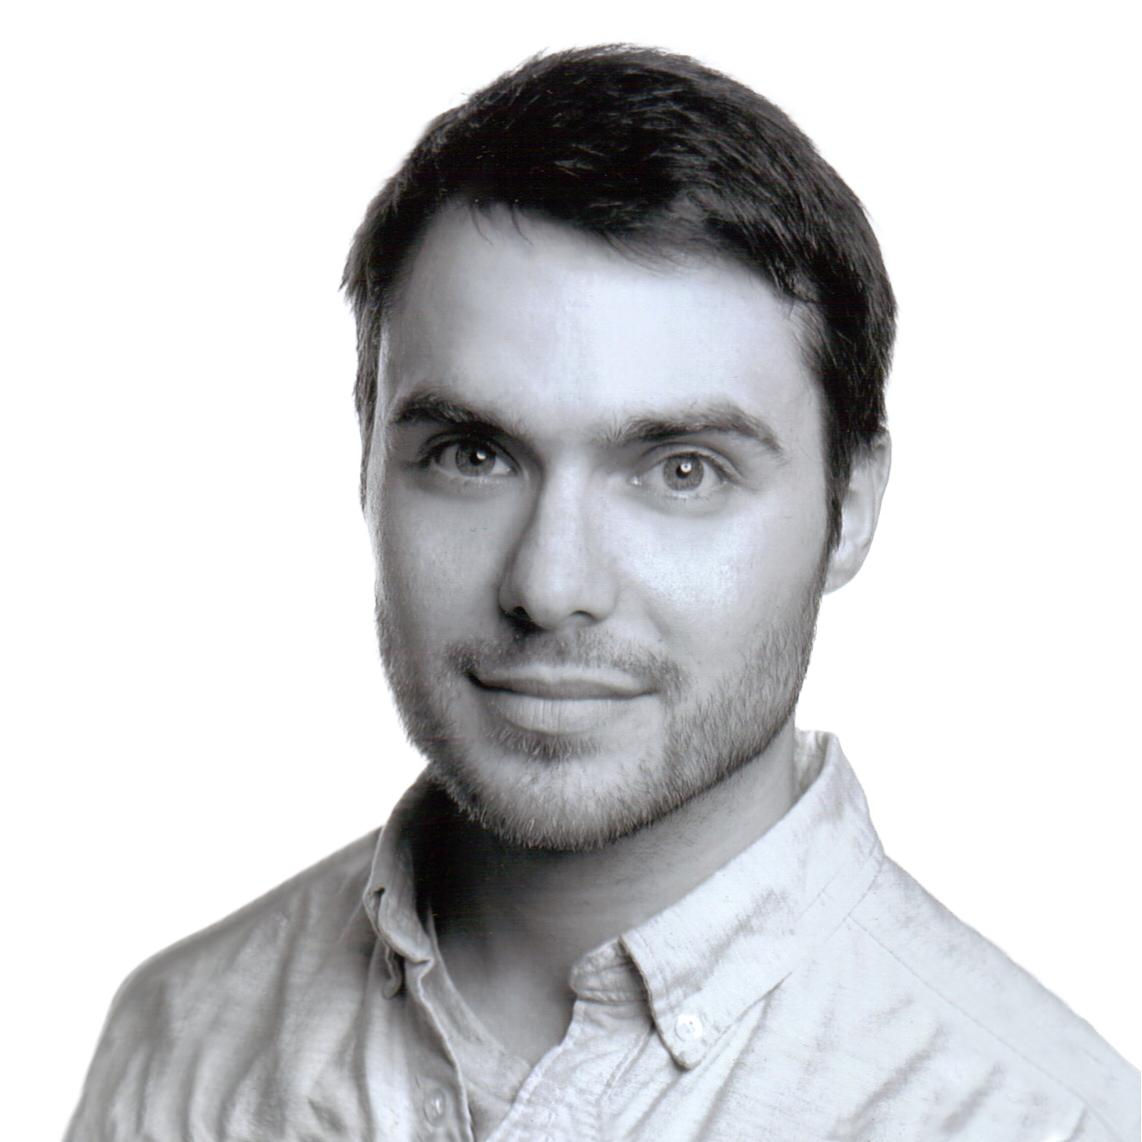
\includegraphics[width=\textwidth]{resources/mug.jpg}
\end{minipage}


\spacedhrule{0.9em}{-0.4em} % Horizontal rule - the first bracket is whitespace before and the second is after

%----------------------------------------------------------------------------------------
%	SUMMARY SECTION
%----------------------------------------------------------------------------------------

\roottitle{Summary} % Root section title

\vspace{-1.3em} % Reduce whitespace after the Summary heading and the two-column content

\begin{multicols}{2}  % Start a two-column layout
\noindent

Sebastian received the Dr.\ rer.\ nat.\ (PhD) degree with distinction (``summa cum laude'') from the Berlin Institute of Technology in 2018.
From 2007 to 2013 he studied computer science (B.\ Sc.\ and M.\ Sc.) at the Berlin Institute of Technology, with a focus on software engineering and machine learning.
Currently, he is a tenured researcher at the machine learning group at Fraunhofer Heinrich Hertz Institute (HHI) in Berlin.
His research interests include computer vision, (efficient) machine learning and data analysis,
data and algorithm visualization, and the interpretation, (meta-)analysis and rectification of machine learning system behavior.

%Besides his professional endeavours, Sebastian enjoys automating repeating office work
\end{multicols}

\spacedhrule{0.5em}{-0.4em} % Horizontal rule - the first bracket is whitespace before and the second is after



%----------------------------------------------------------------------------------------
%	EXPERIENCE SECTION
%----------------------------------------------------------------------------------------

\roottitle{Professional Experience} % Top level section

\headedsection % Employer name which can include a hyperlink and location/URL on the right side of the page
{\href{https://www.hhi.fraunhofer.de/}{Fraunhofer Heinrich Hertz Institute}/\href{https://www.hhi.fraunhofer.de/}{\acr{HHI}}}
{\textsc{Berlin, Germany}}
{

    \headedsubsection % Job title entry for the current employer
    {Tenured Researcher}
    {Jan '19 -- present}
    {
        \bodytext{
            Occupation of a PostDoc position at Fraunhofer HHI.

            \vstep

            \emph{Current research focus:}
            Development of (meta-)analysis methods of machine learning behaviour.
            Improving machine learning predictors and data sources using interpretability feedback.

            %AUTOBIOGRAPHIC TEXT
            %Sebastian currently occupies a PostDoc position at Fraunhofer HHI,
            %with a research focus on interpretability in machine learning.
            %This includes the development of methods for deriving meta-analyses of machine learning system behavior
            %(i.e.\ statistics over large sets of analyses of single predictions),
            %as well as the utilization of model analysis feedback for improving the machine learning predictor or its data source.
        }
    }

    \headedsubsection % Job title entry for the current employer
    {Research Associate}
    {Oct '14 -- Dec '18}
    {
        \bodytext{
            Affiliation to the newly founded machine learning group at Fraunhofer HHI
            with simultaneous continuation of PhD studies at TU Berlin.

            \vstep

            \emph{Research focus:} Applications and refinement of the ``Layer-wise Relevance Propagation'' (LRP) method,
            resulting in several highly cited publications and multiple open source software tools and repositories.

            \vstep

            \emph{Other work:} Extensions of the h.265 (HEVC) video codec towards the upcoming h.266 standard.

            Conceptualization and setup of a HPC cluster with modern GPU hardware.

            Implementation of multiple live demos hands-on showcasing the groups' research nation-wide and internationally.

            \vstep

            Additional supervision by Dr. Wojciech Samek.
            %AUTOBIOGRAPHIC TEXT
            %In continued pursuit of his PhD at TU Berlin, Sebastian affiliates himself to Fraunhofer
            %Hertz Institute as a research associate in the newly founded machine learning group headed by Dr. Wojciech Samek.
            %Research work revolves around applications and the refinement of the
            %``Layer-wise Relevance Propagation'' method,
            %resulting in several highly cited publications and multiple open source software tools and repositories.
            %Other work includes extensions and iterations of the h.265 (HEVC) video codec towards application in the upcoming h.266 standard,
            %the conceptualization and setup of a HPC cluster with modern GPU hardware for the group,
            %as well as the implementation of multiple live demos hands-on showcasing the groups' research nation-wide and internationally.
        }
    }
}

%------------------------------------------------

\headedsection % Employer name which can include a hyperlink and location/URL on the right side of the page
{\href{http://www.tu-berlin.de/ }{Berlin Institute of Technology}/\href{http://www.tu-berlin.de/ }{\acr{TU Berlin}}}
{\textsc{Berlin, Germany}}
{
    \headedsubsection % Job title entry for the current employer
    {Research Associate}
    {Sep '13 -- Sep '14}
    {
        \bodytext{
            \emph{Research focus:}
            Formalization of the ``Layer-wise Relevance Propagation'' (LRP) concept for explaining individual
            and nonlinear decisions of machine learning methods, including Neural Networks and kernelized predictors.

            \vstep

            Extension of LRP to one class learning and anomaly detection tasks.

            \vstep

            Supervision by Prof. Dr. Klaus-Robert M\"uller and Prof. Dr. Alexander Binder.

            %AUTOBIOGRAPHIC TEXT
            %Sebastian spends the first year of his PhD as a research associate in the machine learning department at TU Berlin,
            %which results a general formalization of the ``Layer-wise Relevance Propagation'' (LRP) concept for explaining individual
            %and nonlinear decisions of machine learning methods,
            %including predictors comprised of Deep Neural Networks, kernel machines and arbitrary mapping functions.
            %Applications of LRP also extend to one class learning and anomaly detection tasks on network graph data.
            %Sebastian is supervised by Prof. Dr. Klaus-Robert M\"uller and Prof. Dr. Alexander Binder.
        }
    }

    \headedsubsection % Job title entry for the current employer
    {Research/Teaching Assistant}
    {Oct '11 -- Aug '13}
    {
        \bodytext{

            Research assistant to Prof. Dr. Alexander Binder at the department for machine learning at TU Berlin.

            \emph{Tasks:} Structure and cell type detection in large histopathology images using Bag of Words image processing pipelines and SVM classifiers.

            \vstep

            Teaching assistant to Prof. Dr. Klaus-Robert M\"uller and Prof. Dr. Franz Kir\'aly.

            \emph{Tasks:} Preparation and lecturing of exercise sessions complementing the lectures ``Machine Learning~1'' and ``Machine Learning~2 -- Theory and Application''.

            Visualization and animation of data and learning algorithms discussed in the lecture.
            %AUTOBIOGRAPHIC TEXT
            %During his Master's studies, Sebastian contributes to the machine learning department at TU Berlin
            %as a research assistant and teaching assistant.

            %Sebastian supports Prof. Dr. Alexander Binder in research tasks involving
            %structure and cell type detection in large histopathology images
            %using Bag of Words image processing pipelines and multiple kernel support vector classifiers.

            %As a teaching assistant to Prof. Klaus-Robert M\"uller and Dr. Franz Kir\'aly,
            %Sebastian contributes to the preparation and lecturing of exercise sessions
            %complementing the lectures ``Machine Learning 1'' and ``Machine Learning 2 -- Theory and Application''.
            %He frequently fosters machine learning intuition by providing interactive
            %visualization  and animations of data and learning algorithms discussed in the lecture.
        }
    }

    \headedsubsection % Job title entry for the current employer
    {Teaching Assistant}
    {Oct '09 -- Sep '11}
    {
        \bodytext{

            Teaching assistant to Prof. Dr. Marc Alexa, Prof. Dr. Odej Kao and Prof. Dr. Oliver Brock.

            \emph{Tasks:}
            Course instruction for algorithmic and practical foundations of computer science (B.Sc.).

            \vstep

            \emph{Curriculum:} Basic and advanced Java development, software engineering and OOP concepts, algorithms on image and graph data, among others.

            %AUTOBIOGRAPHIC TEXT
            %Alongside....\todo{continue full text here, if required}
            %Instructor for algorithmic and practical foundations of computer science,
            %covering topics of two semester courses from the B.Sc. Computer Science curriculum at TU Berlin:
            %Basic and advanced Java development, software engineering,
            %graph computations and various computer graphics algorithms, among others.
        }
    }
}

%------------------------------------------------

%\begin{center}
%\textit{Please refer to \href{https://www.linkedin.com/in/sebastian-lapuschkin-903b3b140/}{my Linkedin profile} for the complete list of work experiences along with recommendations.}
%\end{center}

%------------------------------------------------

\spacedhrule{0.5em}{-0.4em} % Horizontal rule - the first bracket is whitespace before and the second is after



%----------------------------------------------------------------------------------------
%	EDUCATION SECTION
%----------------------------------------------------------------------------------------

\roottitle{Education} % Top level section

\headedsection % Employer name which can include a hyperlink and location/URL on the right side of the page
{\href{http://www.tu-berlin.de/ }{Berlin Institute of Technology}/\href{http://www.tu-berlin.de/ }{\acr{TU Berlin}}}
{\textsc{Berlin, Germany}}
{
    \headedsubsection % Job title entry for the current employer
    {PhD in Machine Learning \textnormal{(with distinction / ``summa cum laude'')}}
    {2013 -- 2018}
    {
        \bodytext{
            \emph{Research focus} on methods and applications of \emph{explainable AI (XAI)}:

            Layer-wise Relevance Propagation, Deep Taylor Decomposition, Spectral Relevance Analysis, et cetera.

            \vstep

            20 published and peer-reviewed research papers with
            \href{https://scholar.google.de/citations?user=wpLQuroAAAAJ&hl=de&oi=ao}{over 1500 citations according to Google Scholar}.

            \vstep

            \href{http://dx.doi.org/10.14279/depositonce-7942}{Thesis: ``Opening the machine learning black box with Layer-wise Relevance Propagation''}

            %%AUTOBIOGRAPHIC TEXT
            %My PhD revolves around interpretability in machine learning (or: \emph{explainable AI (XAI)}), which continues the work started with my master's thesis.
            %My co-authors and I formalize and introduce the concept of ``Layer-wise Relevance Propagation'', a widely applicable XAI framework backed up by solid mathematical theory (``Deep Taylor Decomposition'').
            %Using our method, we identify multiple critical flaws in benchmark datasets popular in the computer vision community and multiple (former) state-of-the-art machine learning models.
            %With ``Spectral Relevance Analysis'' we introduce a novel meta analysis framework able to analyze large sets of explanations obtained from XAI methods.

            %%%Layer-wise Relevance Propagation (LRP), Deep Taylor Decomposition (DTD) and Spectral Relevance Analysis (SpRAy)

            %During that time I have submitted and published 20 research papers in high impact journals and conference proceedings reverberating in national and international media.
            %\\
            %\href{http://dx.doi.org/10.14279/depositonce-7942}{Thesis: ``Opening the machine learning black box with Layer-wise Relevance Propagation''}
            }
    }

    \headedsubsection % Job title entry for the current employer
    {Master of Science degree in Computer Science
    % \textnormal{(1.4 / ``very good'' / GPA 3.7)}
    }
    {2010 -- 2013}
    {
        \bodytext{
            Heavy focus on machine learning,
            computer vision and large scale data processing.
            Development dominantly using C++, C\#, Java, Matlab and python.

            \vstep

            My thesis introduces a precursor concept to ``Layer-wise Relevance Propagation'' for interpreting predictions of Bag of Words image processing pipelines with multiple kernel SVMs.

            \vstep

            \href{https://lapuschkin.com/nextcloud/index.php/s/ZgQFsbRBHzRGb9g}{Thesis: ``On Pixel-wise Predictions from Image-wise Bag of Words Classification''} (Grade: 1.0 /  A)
        }
    }

    \headedsubsection % Job title entry for the current employer
    {Bachelor of Science degree in Computer Science
    % \textnormal{(2.0 / ``good'' / GPA 3.0)}
    }
    {2007 -- 2010}
    {
        \bodytext{
            Focus on algorithms, software development and data analysis using imperative (Java, C, C++) and functional (OPAL) programming languages.

            \vstep

            \href{https://lapuschkin.com/nextcloud/index.php/s/8SWord8NAsnMcnn}{Thesis: ``Keyword-Based Image Browsing of Large Image Databases''} (Grade: 1.0 / A)
            }
    }
}

%------------------------------------------------

\headedsection % Employer name which can include a hyperlink and location/URL on the right side of the page
{\href{https://www.deutschhaus.de/ }{Deutschhaus-Gymnasium}/\href{https://www.deutschhaus.de/ }{\acr{DHG}}}
{\textsc{W\"urzburg, Germany}}
{
\headedsubsection % Job title entry for the current employer
{Abitur \textnormal{(pre-university secondary education)}}
{1998 -- 2007}
 {}
}

\spacedhrule{0.5em}{-0.4em} % Horizontal rule - the first bracket is whitespace before and the second is after

%----------------------------------------------------------------------------------------
%	SKILLS SECTION
%----------------------------------------------------------------------------------------

\roottitle{Skills} % Top level section

\inlineheadsection % Special section that has an inline header with a 'hanging' paragraph
{Technical specialties:}
{Extensive experience in software development
using various languages, tools and environments:\\
(bash, C, C++, C\#, git, HTML, Java, LINUX, lua, Matlab, python, subversion, SQL, UNIX, \dots )


Proficiency in scientific working and writing (e.g.\ \LaTeX, Inkscape, \dots),

the development and application of machine learning methods\\
(e.g.\ SVMs, DNNs, preprocessing pipelines, embeddings, clustering, \dots),

in various application domains\\
(text, audio, video, images, time series and biomechanical data, \dots).
}

%------------------------------------------------

\vspace{.65em}
\inlineheadsection % Special section that has an inline header with a 'hanging' paragraph
{Natural languages:}
{German \textit{(mother tongue)}, English \textit{(full professional proficiency)}.}

%------------------------------------------------

\spacedhrule{1.6em}{-0.4em} % Horizontal rule - the first bracket is whitespace before and the second is after

% %----------------------------------------------------------------------------------------
% %	INTERESTS SECTION
% %----------------------------------------------------------------------------------------

% \roottitle{Interests} % Top level section

% \inlineheadsection % Special section that has an inline header with a 'hanging' paragraph
% {In no particular order:}
% {
%     Data visualization,
%     programming,
%     working out,
%     (couch-coop) video games,
%     (audio) books,
%     over-engineered automation of daily tasks,
%     the outdoors and spending time with the wife, dogs \& kid hiking in the woods,
%     vegan food (cooking and eating, much).
% }

% %----------------------------------------------------------------------------------------

% \spacedhrule{1.6em}{-0.4em} % Horizontal rule - the first bracket is whitespace before and the second is after


%----------------------------------------------------------------------------------------
%	AWARDS SECTION
%----------------------------------------------------------------------------------------

\roottitle{Awards} % Top level section

\inlineheadsection % Special section that has an inline header with a 'hanging' paragraph
{Hugo-Geiger-Preis (2020, 1st prize)}
{
    F\"orderpreis f\"ur herausragende Promotionsleistungen
}

\inlineheadsection % Special section that has an inline header with a 'hanging' paragraph
{Freunde des HHI (2019)}
{
    F\"orderpreis f\"ur exzellente wissenschaftliche Arbeiten am HHI
}

\inlineheadsection % Special section that has an inline header with a 'hanging' paragraph
{ERCIM (2019, finalist)}
{
    Cor Baayen Young Researcher Award
}

\inlineheadsection % Special section that has an inline header with a 'hanging' paragraph
{Best Paper Prize (2016)}
{
    ICML'16 Workshop on Visualization for Deep Learning
}

%----------------------------------------------------------------------------------------

\spacedhrule{1.6em}{-0.4em} % Horizontal rule - the first bracket is whitespace before and the second is after



%----------------------------------------------------------------------------------------
%	Patents Section
%----------------------------------------------------------------------------------------

\roottitle{Patents} % Top level section

\inlineheadsection % Special section that has an inline header with a 'hanging' paragraph
{Relevance Score Assignment for Artificial Neural Networks\\}
{
    (submitted 2015)\\
    granted:
    RU 2703343\\
    pending:
    EP 3271863A1, JP 2018513507A, CA 2979579A1, US 15710455

}

%----------------------------------------------------------------------------------------

\spacedhrule{1.6em}{-0.4em} % Horizontal rule - the first bracket is whitespace before and the second is after



%----------------------------------------------------------------------------------------
%	PUBLICATIONS SECTION
%----------------------------------------------------------------------------------------

\roottitle{Publications} % Top level section
%params: 1:authors, 2:year, 3:title, 4:publishedin, 5:pages, 6:link
\newcommand{\journalref}[6]{#1 (#2).\\``#3''.\\In: \href{#6}{\textit{#4} #5}}
%params: 1:authors, 2:year, 3:title, 4:publishedin, 5:pages, 6:link
\newcommand{\conferenceref}[6]{#1 (#2).\\``#3''.\\In: \href{#6}{\textit{#4} #5}}
%params: 1:authors, 2:year, 3:title, 4:publishedin, 5:pages, 6:link, 7:note
\newcommand{\conferencerefwnote}[7]{#1 (#2).\\``#3''.\\In: \href{#6}{\textit{#4} #5}. \textit{#7} }
%params: 1:authors, 2:year, 3:title, 4:publishedin, 5:pages, 6:link, 7:publisher
\newcommand{\bookchapterref}[7]{#1 (#2).\\``#3''.\\In: \href{#6}{\textit{#4} #5}. #7}
%params: 1:authors, 2:year, 3:title, 4:publishedin, 5:link
\newcommand{\preprintref}[5]{#1 (#2).\\``#3''.\\In: \href{#5}{\textit{#4}}}
%params: 1:authors, 2:year, 3:title, 4:publishedin, 5:link, 6:note
\newcommand{\preprintrefwnote}[6]{#1 (#2).\\``#3''.\\In: \href{#5}{\textit{#4}}. \textit{#6}}

\headedsection % Employer name which can include a hyperlink and location/URL on the right side of the page
{Journal Articles}{ }
{
\begin{enumerate}
    \item[] \journalref{Alber M, \textbf{Lapuschkin S}, Seegerer P, H\"agele M, Sch\"utt K T, Montavon G, Samek W, M\"uller K-R, D\"ahne S and Kindermans P-J}
                        {2019}
                        {iNNvestigate Neural Networks!}
                        {Journal of Machine Learning Research}
                        {20(93):1-8}
                        {http://jmlr.org/papers/v20/18-540.html}

    \item[] \journalref{\textbf{Lapuschkin S}, W\"aldchen S, Binder A, Montavon G, Samek W and M\"uller K-R}
                        {2019}
                        {Unmasking Clever Hans Predictors and Assessing what Machines Really Learn}
                        {Nature Communications}
                        {10:1069}
                        {https://doi.org/10.1038/s41467-019-08987-4}

    \item[] \journalref{Horst F, \textbf{Lapuschkin S}, Samek W, M\"uller K-R and Sch\"ollhorn W I}
                        {2019}
                        {Explaining the Unique Nature of Individual Gait Patterns with Deep Learning}
                        {Scientific Reports}
                        {9:2391}
                        {https://doi.org/10.1038/s41598-019-38748-8}

    \item[] \journalref{Montavon G, \textbf{Lapuschkin S}, Binder A, Samek W and M\"uller K-R}
                        {2017}
                        {Explaining NonLinear Classification Decisions with Deep Taylor Decomposition}
                        {Pattern Recognition}
                        {65:211-222}
                        {https://doi.org/10.1016/j.patcog.2016.11.008}

    \item[] \journalref{Samek W, Binder A, Montavon G, \textbf{Lapuschkin S}, and M\"uller K-R}
                        {2017}
                        {Evaluating the Visualization of what a Deep Neural Network has Learned}
                        {IEEE Transactions of Neural Networks and Learning Systems}
                        {}
                        {https://doi.org/10.1109/TNNLS.2016.2599820}

    \item[] \journalref{Sturm I, \textbf{Lapuschkin S}, Samek W and M\"uller K-R}
                        {2016}
                        {Interpretable Deep Neural Networks for Single-Trial EEG Classification}
                        {Journal of Neuroscience Methods}
                        {274:141-145}
                        {https://doi.org/10.1016/j.jneumeth.2016.10.008}

    \item[] \journalref{\textbf{Lapuschkin S}, Binder A, Montavon G, M\"uller K-R and Samek W}
                        {2016}
                        {The Layer-wise Relevance Propagation Toolbox for Artificial Neural Networks}
                        {Journal of Machine Learning Research}
                        {17(114):1-5}
                        {http://www.jmlr.org/papers/v17/15-618.html}

    \item[] \journalref{\textbf{Bach S}, Binder A, Montavon G, Klauschen F, M\"uller K-R and Samek W}
                        {2015}
                        {On Pixel-wise Explanations for Non-Linear Classifier Decisions by Layer-wise Relevance Propagation}
                        {PLoS ONE}
                        {10(7):e0130140}
                        {https://doi.org/10.1371/journal.pone.0130140}
\end{enumerate}
}

%------------------------------------------------
\headedsection % Employer name which can include a hyperlink and location/URL on the right side of the page
{Contributions to Conference Proceedings}{}
{
    \begin{enumerate}
        \item[] \conferenceref{Alber M, \textbf{Lapuschkin S}, Seegerer P, H\"agele M, Sch\"utt K T, Montavon G, Samek W, M\"uller K-R, D\"ahne S and Kindermans P-J}
                                {2018}
                                {How to iNNvestigate Neural Networks' Predictors!}
                                {Machine Learning Open Source Software: Sustainable Communities. NIPS Workshop}
                                {}
                                {https://openreview.net/forum?id=ByeDpyc0Ym}


        \item[] \conferenceref{\textbf{Lapuschkin S}, Binder A, M\"uller K-R and Samek W}
                                {2017}
                                {Understanding and Comparing Deep Neural Networks for Age and Gender Classification}
                                {Proceedings of the ICCV'17 Workshop on Analysis and Modeling of Faces and Gestures (AMFG)}
                                {2017:1629-1638}
                                {https://doi.org/10.1109/ICCVW.2017.191}
                                %{Poster + Oral + Live demo}

        \item[] \conferenceref{Srinivasan V, \textbf{Lapuschkin S}, Hellge C, M\"uller K-R and Samek W}
                                {2017}
                                {Interpretable Action Recognition in Compressed Domain}
                                {Proceedings of the IEEE International Conference on Acoustics, Speech and Signal Processing (ICASSP)}
                                {2017:1692-1696}
                                {https://doi.org/10.1109/ICASSP.2017.7952445}


        \item[] \conferenceref{\textbf{Bach S}, Binder A, M\"uller K-R and Samek W}
                                {2016}
                                {Controlling Explanatory Heatmap Resolution and Semantics via Decomposition Depth}
                                {Proceedings of the IEEE International Conference of Image Processing (ICIP)}
                                {2016:2271-2275}
                                {https://doi.org/10.1109/ICIP.2016.7532763}


        \item[] \conferencerefwnote{Binder A, Samek W, Montavon G, \textbf{Bach S}, and M\"uller K-R}
                                {2016}
                                {Analyzing and Validating Neural Network Predictions}
                                {Proceedings of the ICML'16 Workshop on Visualization for Deep Learning}
                                {}
                                {http://iphome.hhi.de/samek/pdf/BinICML16.pdf}
                                {Best paper award winner}

        \item[] \conferenceref{\textbf{Lapuschkin S}, Binder A, Montavon G, M\"uller K-R and Samek W}
                                {2016}
                                {Analyzing Classifiers: Fisher Vectors and Deep Neural Networks}
                                {Proceedings of the IEEE Conference on Computer Vision and Pattern Recognition (CVPR)}
                                {2016:2912-2920}
                                {https://doi.org/10.1109/CVPR.2016.318}

        \item[] \conferenceref{Montavon G, \textbf{Bach S}, Binder A, Samek W and M\"uller K-R}
                                {2016}
                                {Deep Taylor Decomposition of Neural Networks}
                                {Proceedings of the ICML'16 Workshop on Visualization for Deep Learning}
                                {2016:2912-2920}
                                {http://iphome.hhi.de/samek/pdf/MonICML16.pdf}

        \item[] \conferenceref{Samek W, Montavon G, Binder A, \textbf{Lapuschkin S} and M\"uller K-R}
                                {2016}
                                {Interpreting the Predictions of Complex ML Models by Layer-wise Relevance Propagation}
                                {Proceedings of the Interpretable ML for Complex Systems NIPS'16 Workshop}
                                {}
                                {http://iphome.hhi.de/samek/pdf/SamNIPS16.pdf}

    \end{enumerate}
}

%------------------------------------------------

\headedsection % Employer name which can include a hyperlink and location/URL on the right side of the page
{Book Chapters}{}
{
    \begin{enumerate}
        \item[] \bookchapterref{Montavon G, Binder A, \textbf{Lapuschkin S}, Samek W and M\"uller K-R}
                            {2019}
                            {Layer-wise relevance propagation: An Overview}
                            {Explainable AI: Interpreting, Explaining and Visualizing Deep Learning}
                            {193-209}
                            {https://doi.org/10.1007/978-3-030-28954-6_10}
                            {Springer, Cham}

        \item[] \bookchapterref{Binder A, \textbf{Bach S}, Montavon G, M\"uller K-R and Samek W}
                            {2016}
                            {Layer-wise Relevance Propagation for Deep Neural Network Architectures}
                            {Information Science and Applications (ICISA) 2016. Lecture Notes in Electrical Engineering}
                            {276:913-922}
                            {https://doi.org/10.1007/978-981-10-0557-2_87}
                            {Springer, Singapore}

        \item[] \bookchapterref{Binder A, Montavon G, \textbf{Lapuschkin S}, M\"uller K-R and Samek W}
                            {2016}
                            {Layer-wise Relevance Propagation for Neural Networks with Local Renormalization Layers}
                            {Lecture Notes in Computer Science}
                            {9887:63-71}
                            {https://doi.org/10.1007/978-3-319-44781-0_8}
                            {Springer, Berlin/Heidelberg}
    \end{enumerate}

}

%------------------------------------------------
\clearpage
\headedsection % Employer name which can include a hyperlink and location/URL on the right side of the page
{Preprints}{}
{
    \begin{enumerate}
        \item[] \preprintref{Sun J, \textbf{Lapuschkin S}, Samek W and Binder A}
                            {2020}
                            {Understanding Image Captioning Models beyond Visualizing Attention}
                            {CoRR abs/2001.01037}
                            {https://arxiv.org/abs/2001.01037}

        \item[] \preprintref{Anders C J, Marin\v{c} T, Neumann D, Samek W, M\"uller K-R and \textbf{Lapuschkin S}}
                            {2019}
                            {Analyzing ImageNet with Spectral Relevance Analysis: Towards ImageNet un-Hans'ed}
                            {CoRR abs/1912.11425}
                            {https://arxiv.org/abs/1912.11425}

        \item[] \preprintref{Yeom S-K, Seegerer P, \textbf{Lapuschkin S}, Wiedemann S, M\"uller K-R and Samek W}
                            {2019}
                            {Pruning by Explaining: A Novel Criterion for Deep Neural Network Pruning}
                            {CoRR abs/1912.08881}
                            {https://arxiv.org/abs/1912.08881}

        \item[] \preprintref{Horst F, Slijepcevic D, \textbf{Lapuschkin S}, Raberger A-M, Zeppelzauer M, Samek W, Breiteneder C, Sch\"ollhorn W I and Horsak B}
                            {2019}
                            {On the Understanding and Interpretation of Machine Learning Predictions in Clinical Gait Analysis Using Explainable Artificial Intelligence}
                            {CoRR abs/1912.07737}
                            {https://arxiv.org/abs/1912.07737}

        \item[] \preprintref{Kohlbrenner M, Bauer A, Nakajima S, Binder A, Samek W and \textbf{Lapuschkin S}}
                            {2019}
                            {Towards Best Practice in Explaining Neural Network Decisions with LRP}
                            {CoRR abs/1910.09840}
                            {https://arxiv.org/pdf/1910.09840}


        \item[] \preprintref{H\"agele M, Seegerer P, \textbf{Lapuschkin S}, Bockmayr M, Samek W, Klauschen F, M\"uller K-R and Binder A}
                            {2019}
                            {Resolving Challenges in Deep Learning-based Analyses of Histopathological Images using Explanation Methods}
                            {CoRR abs/1908.06943}
                            {https://arxiv.org/abs/1908.06943}

        \item[] \preprintref{Becker S, Ackermann M, \textbf{Lapuschkin S}, M\"uller K-R and Samek W}
                            {2018}
                            {Interpreting and Explaining Deep Neural Networks for Classification of Audio Signals}
                            {CoRR abs/1807.03418}
                            {https://arxiv.org/abs/1807.03418}

        \item[] \preprintref{Schwenk G and \textbf{Bach S}}
                            {2014}
                            {Detecting Behavioural and Structural Anomalies in Media-Cloud Applications}
                            {CoRR abs/1409.8035}
                            {https://arxiv.org/abs/1409.8035}

    \end{enumerate}

}


\end{document}
